%%%%%%%%%%%%%%%%%%%%%%%%%%%%%%%%%%%%%%%%%%%%%%%%%%%%%%%
\mychapter{Questões paramétricas}\label{ch:questoesCodigoMCTest}

No capítulo anterior, foi apresentada a criação de questões estáticas de múltipla escolha (QMs) e dissertativas (QTs), incluindo uma questão típica utilizada em disciplinas de lógica de programação na UFABC, apresentada na Figura \ref{fig:cap04_figQuestaoAtualizaPDF4}. É possível criar essas questões utilizando \LaTeX, uma linguagem de preparação de documentos de alta qualidade e profissionalismo, com recursos avançados para controle de tipos de letra, espaçamento, numeração de seções, referências bibliográficas e equações matemáticas, entre outros. \LaTeX{} é gratuita e está disponível para vários sistemas operacionais.

A linguagem \LaTeX{} foi criada no início da década de 1980 pelo matemático e cientista da computação Leslie Lamport \cite{lamport1985latex}. Ela é baseada no \TeX, uma linguagem de marcação desenvolvida por Donald Knuth na década de 1970 para produzir documentos com alta qualidade tipográfica para sua série de livros ``\textit{The Art of Computer Programming}''. O \TeX{} se tornou popular para a produção de documentos científicos, técnicos e matemáticos e ainda é amplamente utilizado atualmente.

Para contornar a sintaxe complexa e de difícil programação do \LaTeX{}, no MCTest foi introduzida a possibilidade de intercalar trechos em \LaTeX{} com trechos de código em Python. Python é uma linguagem de programação de alto nível, interpretada e de propósito geral, criada no início da década de 1990 por Guido van Rossum, e atualmente é uma das linguagens de programação mais populares do mundo~\footnote{Levantamento das linguagens de programação mais populares em 2023: \href{https://survey.stackoverflow.co/2023}{survey.stackoverflow.co/2023} e  \href{https://pypl.github.io/PYPL.html}{pypl.github.io/PYPL.html}.}. Com uma ampla variedade de aplicações em áreas como desenvolvimento web, ciência de dados, inteligência artificial e automação de processos, Python é conhecida por sua sintaxe clara e legível, facilitando a escrita e a leitura de código. 

O MCTest proporciona aos usuários a capacidade de criar questões diversas e paramétricas, combinando o uso do formato \LaTeX{} e da linguagem de programação Python. Essa funcionalidade será apresentada neste capítulo. Em capítulos futuros, na Parte - \ref{part:experimentos} - \textbf{Experimentos}, serão exploradas com mais detalhes essa característica fundamental do MCTest de criar questões paramétricas.
%
Essa abordagem proporciona maior flexibilidade na criação de questões personalizadas e permite uma fácil manipulação dos parâmetros definidos pelos professores. Dessa forma, a criação de questões torna-se mais eficiente e adaptável às necessidades específicas de cada disciplina.

Apesar dessa possibilidade, muitas vezes a criação de questões paramétricas ainda exige habilidades de programação por parte do professor. No entanto, quando há um grupo de professores interessados e uma grande demanda de avaliações para milhares de estudantes, o MCTest oferece a gestão de avaliações utilizando um banco de questões que podem ser facilmente reaproveitadas em avaliações futuras. Essa abordagem já foi avaliada em várias publicações científicas, demonstrando eficiência e eficácia em avaliações, como apresentado em \href{http://vision.ufabc.edu.br}{vision.ufabc.edu.br}. 

\section{QM paramétrica}

A criação de QMs é uma tarefa comum para professores de diversas áreas do conhecimento. Para tornar esse processo mais eficiente, é possível utilizar recursos de programação. Nesta seção, será abordada a QM paramétrica, que permite criar questões com variações de parâmetros. Isso possibilita a criação de inúmeras questões com facilidade e rapidez. Serão apresentados exemplos de como criar questões paramétricas em Python, utilizando o MCTest como plataforma. Serão abordadas diferentes técnicas de parametrização, permitindo ao professor escolher a que melhor se adapta à sua habilidade em programação.


\subsection{Um exemplo}

Suponha que você seja um professor de matemática e deseje criar várias QMs sobre a fórmula da área do círculo. Embora este exemplo seja bastante simples, é possível generalizar para questões mais complexas. Para alcançar esse objetivo, você pode utilizar o seguinte método em Python:


\begin{listing}[!ht]
\begin{myboxCode}{corCodigo}{\textbf{Código: } método \verb|area_circulo(raio)|}\vspace{3mm}
\hrule
\begin{minted}[xleftmargin=20pt,linenos=true]{python}
import math

def area_circulo(raio):
  return math.pi * raio ** 2
\end{minted}
\end{myboxCode}
\caption{Exemplo de método para calcular a área de um círculo.}
\label{lst:codigoAreaCirculo}
\end{listing}


Com base no método apresentado no Código \ref{lst:codigoAreaCirculo}, é possível gerar diversas QMs sobre a área do círculo, com as seguintes variações:

\begin{enumerate}
\item A questão deve ter 4 alternativas de resposta;
\item O raio do círculo deve variar aleatoriamente;
\item A alternativa correta deve ser calculada com base no valor do raio;
\item As demais alternativas erradas devem ter valores distintos.
\end{enumerate}

A seguir, serão apresentados três exemplos de questões para calcular a área do círculo, com raios escolhidos aleatoriamente:

\begin{description}
    
    \item \textbf{1) Qual é a área do círculo de raio 2?}

\begin{multicols}{4}
\begin{enumerate}[label=\Alph*.]
\item 3,14
\item 6,28
\item 12,56
\item 25,12
\end{enumerate}
\end{multicols}

    \item \textbf{2) Qual é a área do círculo de raio 4?}

\begin{multicols}{4}
\begin{enumerate}[label=\Alph*.]
\itemsep0pt\parskip0pt\parsep0pt
\item 12,56
\item 25,12
\item 37,68
\item 50,24
\end{enumerate}\normalsize
\end{multicols}

    \item \textbf{3) Qual é a área do círculo de raio 3?}

\begin{multicols}{4}
\begin{enumerate}[label=\Alph*.]
\itemsep0pt\parskip0pt\parsep0pt
\item 9,42
\item 12,56
\item 15,70
\item 18,84
\end{enumerate}\normalsize
\end{multicols}

\end{description}


Nos exemplos ilustrativos apresentados, o método \verb|area_circulo| pode ser utilizado para calcular a resposta correta para cada alternativa de resposta. A variação aleatória do raio pode ser realizada com a ajuda da biblioteca \verb|random| do Python. Por fim, as alternativas erradas podem ser calculadas, também utilizando o método \verb|area_circulo|, com base no valor do raio, garantindo a não repetição de alternativas. A seguir, será apresentado esse exemplo implementado no MCTest.

\subsection{QM paramétrica no MCTest}\label{sec:QMparametrica}

É possível parametrizar QMs no MCTest de várias maneiras, dependendo das habilidades de programação em Python do professor. Algumas dessas maneiras são apresentadas nesta seção.

\begin{mybox}{corObs}{\textbf{Observações:\\\vspace{-3mm}\hrule\vspace{1mm}}}
\begin{enumerate}
    \item A descrição da questão no MCTest (campo ``Descrição'' na Figura \ref{fig:cap04_figQuestaoAtualiza}), que pode incluir textos em \LaTeX{} integrados com códigos em Python, é a parte mais importante na criação de questões paramétricas. A partir deste capítulo, não será mais apresentada uma captura de tela da questão, como foram realizados nos dois capítulos anteriores. Para criar uma QM ou QT paramétrica basta alterar o parâmetro ``Paramétrica'' de ``Não'' para ``Sim'', nas telas de criação ou alteração de questão;
    \item A parte mais complicada na criação de questões paramétricas no MCTest é lidar com possíveis erros que podem ser retornados pelo MCTest ao tentar criar o PDF. Para tentar resolver esse problema, foi criado um \textit{notebook} no Google Colab, acessado ao clicar no botão ``Compile-Colab'' nas telas de alteração de questão, como apresentado na Figura \ref{fig:cap04_figQuestaoAtualiza}.
\end{enumerate}
\end{mybox}

\subsubsection{Exemplo 1}

Veja uma descrição da questão paramétrica para calcular a área de um círculo, implementada no MCTest, no Código \ref{lst:questaoQM_AreaCirculoEx1}. Todo o texto que aparece até a linha 6, contendo \verb|[[def:|, fará parte do enunciado da questão e pode utilizar a sintaxe do \LaTeX. As partes paramétricas deste enunciado ocorrem nas instruções em Python entre as marcações \verb|[[code:| e \verb|]]|. Geralmente, essas instruções são variáveis definidas em Python entre as marcações \verb|[[def:| e \verb|]]|, neste exemplo, entre as linhas 6 e 30.

\begin{mybox}{corCopia}{\textbf{Marcações principais definidas no MCTest:\\\vspace{-3mm}\hrule\vspace{1mm}}}
\begin{enumerate}
    \item Instruções que podem representar a parte paramétrica do enunciado da questão ou das alternativas são colocadas entre as marcações \verb|[[code:| e \verb|]]|, conforme exemplificado na linha 1 do Código \ref{lst:questaoQM_AreaCirculoEx1};
    \item Após esse enunciado, um único bloco de código em Python deve ser definido entre as marcações \verb|[[def:| e \verb|]]|, como ilustrado entre as linhas 6 e 30 do exemplo. Todo o texto após esse bloco é descartado do enunciado da questão.
\end{enumerate}
\end{mybox}

\begin{mybox}{corEdicao2}{\textbf{Destaque:\\\vspace{-3mm}\hrule\vspace{3mm}}}
Em alguns casos, ocorre um erro no retorno da expressão regular para capturar as variáveis ou instruções delimitadas por \verb|[[code:| e \verb|]]|. Nesses casos, é necessário adicionar um espaço antes de \verb|[[code:| e após \verb|]]|. O método \verb|get_code| disponível no GitHub em \href{https://github.com/fzampirolli/mctest/blob/master/topic/UtilsMCTest4.py}{UtilsMCTest4.py} propõe uma sugestão de modificação na expressão regular. No entanto, essa sugestão apresenta uma falha quando ocorre uma sequência de \verb|]]| dentro de \verb|[[def:| e \verb|]]|. Assim, para evitar problemas, use sempre espaços antes de \verb|[[code:| e após \verb|]]|.
\end{mybox}

Se as marcações de início e fim de bloco ou instruções aparecerem erroneamente, ou se houver algum erro no código Python, mensagens de erro do compilador Python poderão ser exibidas, mas sem fornecer muitos detalhes sobre o erro específico. Portanto, é fundamental testar o código Python fora do MCTest, por exemplo, utilizando o \textit{notebook} do Google Colab. Para acessar o \textit{notebook}, basta clicar no botão ``Compile-Colab'' nas telas de alteração de questão, como mostrado na Figura \ref{fig:cap04_figQuestaoAtualiza}. Experimente adicionar espaços inesperados, como \verb|[[code: raio1]]| ou \verb|[ [code:raio1]]|, salve e clique em ``Cria-PDF''. Isso permitirá identificar erros e depurar a questão no MCTest, seguindo os seguintes exemplos:

\begin{myboxCode}{corObs}{\textbf{Alguns exemplos de erros comuns que podem ocorrer:\\\vspace{-3mm}\hrule\vspace{3mm}}}
Experimente incluir esses erros, salve e crie o PDF para identificar e corrigir possíveis problemas futuros:
\begin{enumerate}
    \item \verb|[[code: raio1]]| -- espaço não esperado -- retorna:\\ 
    \verb|ERROR in [[code: ... ]]: unmatched ’]’ (<string>, line 1) raio1]]?|
    
    \item \verb|[[code:Raio1]]| -- ``R'' maiúsculo -- retorna:\\
    \verb|ERROR in [[code: ... ]]: name ’Raio1’ is not defined Raio1|
    
    \item Bloco de código no método \verb|area_circulo| sem \textit{identação} correta -- retorna:\\
    \verb|ERROR in [[def: ... ]]: unexpected indent (<string>, line 7)|
    
    \item Sem a linha \verb|import math| no método \verb|area_circulo| -- retorna:\\
    \verb|ERROR in [[def: ... ]]: name ’math’ is not defined|
    
    \item Sem os ``:'' no final da linha do método  \verb|area_circulo| -- retorna:\\
    \verb|ERROR in [[def: ... ]]: invalid syntax (<string>, line 5)|
    
    \item \verb|[ [def:| ou  \verb|[[def :|  -- espaço não esperado -- retorna:\\
    \verb|ERROR in [[code: ... ]]: name ’raio1’ is not defined raio1| 
    
\end{enumerate}
\end{myboxCode}

Observe que, nesse sexto caso, o erro retornado é que a variável \verb|raio1| não foi definida. Isso ocorreu porque o MCTest não encontrou o bloco de código Python entre as marcações \verb|[[def:| e \verb|]]|. Certifique-se de ter incluído corretamente o bloco de código necessário para definir a variável \verb|raio1| e verifique se não há erros de digitação ou formatação nas marcações. Essa etapa é crucial para garantir o funcionamento correto da questão paramétrica no MCTest.

\begin{listing}[!ht]
\begin{myboxCode}{corCodigo}{\textbf{Questão: }}\vspace{3mm}
\hrule
\begin{minted}[xleftmargin=20pt,linenos=true]{python}
Qual é a área do círculo de raio [[code:raio1]]?

% comentário em LaTeX. Observe que a variável raio1, após "code:" 
% foi definida na linha 15 abaixo

[[def: # comentário em Python
# o bloco de código Python deve sempre iniciar com a linha anterior!
import random

def area_circulo(raio): # método para calcular a área do círculo
    import math # necessário importar biblioteca(s) no método
    return math.pi * raio ** 2

# lista de 4 raios aleatórios entre 20 e 50
raio1,raio2,raio3,raio4 = random.sample(range(20,51), 4)

# formata as áreas com 2 casas decimais
area1 = f"{area_circulo(raio1):.2f}"
area2 = f"{area_circulo(raio2):.2f}"
area3 = f"{area_circulo(raio3):.2f}"
area4 = f"{area_circulo(raio4):.2f}"

# incluir nas alternativas:
# [[code:area1]]
# [[code:area2]]
# [[code:area3]]
# [[code:area4]]

# o bloco de código Python deve sempre terminar com a próxima linha
]]
Todo o texto que aparece após a linha anterior é ignorado.
\end{minted}
\end{myboxCode}
\caption{Exemplo de QM paramétrica para calcular a área do círculo.}
\label{lst:questaoQM_AreaCirculoEx1}
\end{listing}


\subsubsection{Exemplo 2}\label{sec:QMparametricaEx2}

Quando as alternativas de uma QM paramétrica assumem apenas valores inteiros, é possível utilizar o método \verb|createWrongAnswers| desenvolvido e disponibilizado no MCTest. No entanto, algumas exigências são necessárias, como apresentado no Código \ref{lst:questaoQM_AreaCirculoEx2}. 

Primeiramente, é necessário criar uma variável global chamada \verb|correctAnswer|, conforme mostrado na linha 12 do código. Em seguida, atribui-se a resposta correta a essa variável, como ilustrado na linha 14. 

No que diz respeito às alternativas da questão, é importante incluir na primeira alternativa o conteúdo da linha 17, sem o comentário. Na segunda alternativa, deve-se utilizar o conteúdo da linha 18, também sem o comentário. Na linha 18, o método irá gerar três valores aleatórios distintos entre \verb|correctAnswer|$-10$ e \verb|correctAnswer|$+10$. 

É importante observar que, nesse caso, as questões geradas não são consideradas ``ótimas'', pois os estudantes podem deduzir que a resposta correta não está nos extremos dos valores fornecidos, conforme ilustrado na Figura \ref{fig:cap05_questaoQM_AreaCirculoPDF}. 
Em QMs, o texto em verde (\verb|#2450|) representa a identificação da questão no banco de dados. Azul (\verb|#0|) representa a primeira alternativa na tela de criação ou alteração da questão. As demais alternativas em vermelho (\verb|*1|, \verb|*2| e \verb|*3|) são as três alternativas erradas criadas pelo método \verb|createWrongAnswers|.


\begin{listing}[!ht]
\begin{myboxCode}{corCodigo}{\textbf{Questão: }}\vspace{3mm}
\hrule
\begin{minted}[xleftmargin=20pt,linenos=true]{python}
Qual é a área do círculo de raio [[code:raio1]]?

[[def:
import random

def area_circulo(raio): 
    import math # necessário importar biblioteca(s) no método
    return math.pi * raio ** 2

raio1 = random.randint(10, 51) # sorteia valor entre 10 e 50

global correctAnswer # variável necessária para usar o método 
# createWrongAnswers, a resposta deve ter valor inteiro
correctAnswer = int(area_circulo(raio1)) 

# incluir nas alternativas da questão: 
# [[code:correctAnswer]] % primeira alternativa (sempre) correta
# [[code:createWrongAnswers([3,10])]] % cria 3 alter. erradas +/- 10
]]
\end{minted}
\end{myboxCode}
\caption{Exemplo de QM paramétrica para calcular a área do círculo, utilizando o método \texttt{createWrongAnswers}.}
\label{lst:questaoQM_AreaCirculoEx2}
\end{listing}

\begin{figure}[!ht]
  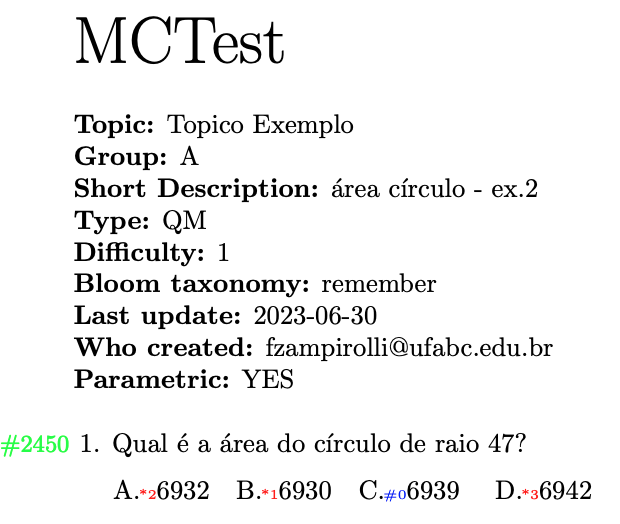
\includegraphics[width=0.5\textwidth]{cap05_questaoQM_AreaCirculoPDF.png}
  \caption{Recorte do PDF gerado para a questão definida no Código \ref{lst:questaoQM_AreaCirculoEx2}.}
  \label{fig:cap05_questaoQM_AreaCirculoPDF}
\end{figure}


\section{QT paramétrica}

Os conceitos apresentados anteriormente para as QMs paramétricas são aplicáveis também às QTs paramétricas, com a distinção de que não há necessidade de considerar as alternativas da questão. Em vez disso, é possível definir uma única resposta correta, se necessário. Nesta seção, serão fornecidos três exemplos adicionais da questão de teste de mesa introduzida no capítulo anterior (Seção \ref{sec:introducaoTextoQT} -- \nameref{sec:introducaoTextoQT}), agora sob a perspectiva paramétrica.

No primeiro exemplo, foi criada uma questão com três parâmetros aleatórios. No segundo exemplo, foi adicionado um gabarito para esses parâmetros aleatórios, implementando a solução do pseudocódigo apresentado em Python e adicionando comandos \verb|print| em locais estratégicos para imprimir a tabela com o gabarito. Por fim, no último exemplo, foi utilizado um recurso avançado de rastreamento de instruções, métodos e exceções.
%
Esses exemplos mostram o poder da parametrização no MCTest para criar questões personalizadas e detalhadas.

\subsection{Exemplo 1 -- Teste de mesa}

Nesta seção, será abordada a parametrização da questão de teste de mesa ilustrada na Figura \ref{fig:cap05_questaoQT_TesteMesaEx2PDF} e apresentada no Código \ref{lst:questaoQT_TesteMesaEx2}, para exemplificar o processo. As partes paramétricas estão localizadas nas linhas 7, 8 e 9 da questão, com os parâmetros \verb|N1|, \verb|N2| e \verb|N3|, cujos valores são definidos aleatoriamente no bloco de código Python nas linhas 38, 39 e 40, respectivamente. O PDF correspondente a essa questão é apresentado na Figura \ref{fig:cap05_questaoQT_TesteMesaEx2PDF}.




\begin{listing}[!ht]
\begin{myboxCode}{corCodigo}{\textbf{Questão: }}\vspace{3mm}
\hrule
\begin{minted}[xleftmargin=20pt,linenos=true]{python}
Preencha a tabela com os valores corretos das variáveis contador e soma 
em cada iteração do laço.  Além disso, considere os números das linhas do 
código para preencher a tabela, a fim de facilitar a referência. Considere 
inicialmente N=[[code:N1]], contador=[[code:N2]] e soma=[[code:N3]].

\begin{verbatim}
1. Inicializar a variável N com [[code:N1]]
2. Inicializar a variável contador com [[code:N2]]
3. Inicializar a variável soma com [[code:N3]]
4. Enquanto contador <= N faça
5.     Se contador é par então
6.         soma = soma + contador
7.     Senão
8.         soma = soma - contador
9.     Fim se
10.    Incrementar contador em 1
11. Fim enquanto
12. Imprimir o valor da variável soma
\end{verbatim}

\begin{tabular}{|c|c|c|c|}
\hline
\textbf{linha} & \textbf{contador} & \textbf{soma} \\
\hline
 & & \\ \hline
 & & \\ \hline
 & & \\ \hline
 & & \\ \hline
 & & \\ \hline
 & & \\ \hline
 & & \\ \hline
 & & \\ \hline
 & & \\ \hline
\end{tabular}

[[def:
import random
N1 = random.randint(7,16)
N2 = random.randint(1,6)
N3 = random.randint(1,5)
]]
\end{minted}
\end{myboxCode}
\caption{Exemplo simples de descrição de QT paramétrica para teste de mesa.}
\label{lst:questaoQT_TesteMesaEx2}
\end{listing}

\begin{figure}[!ht]
  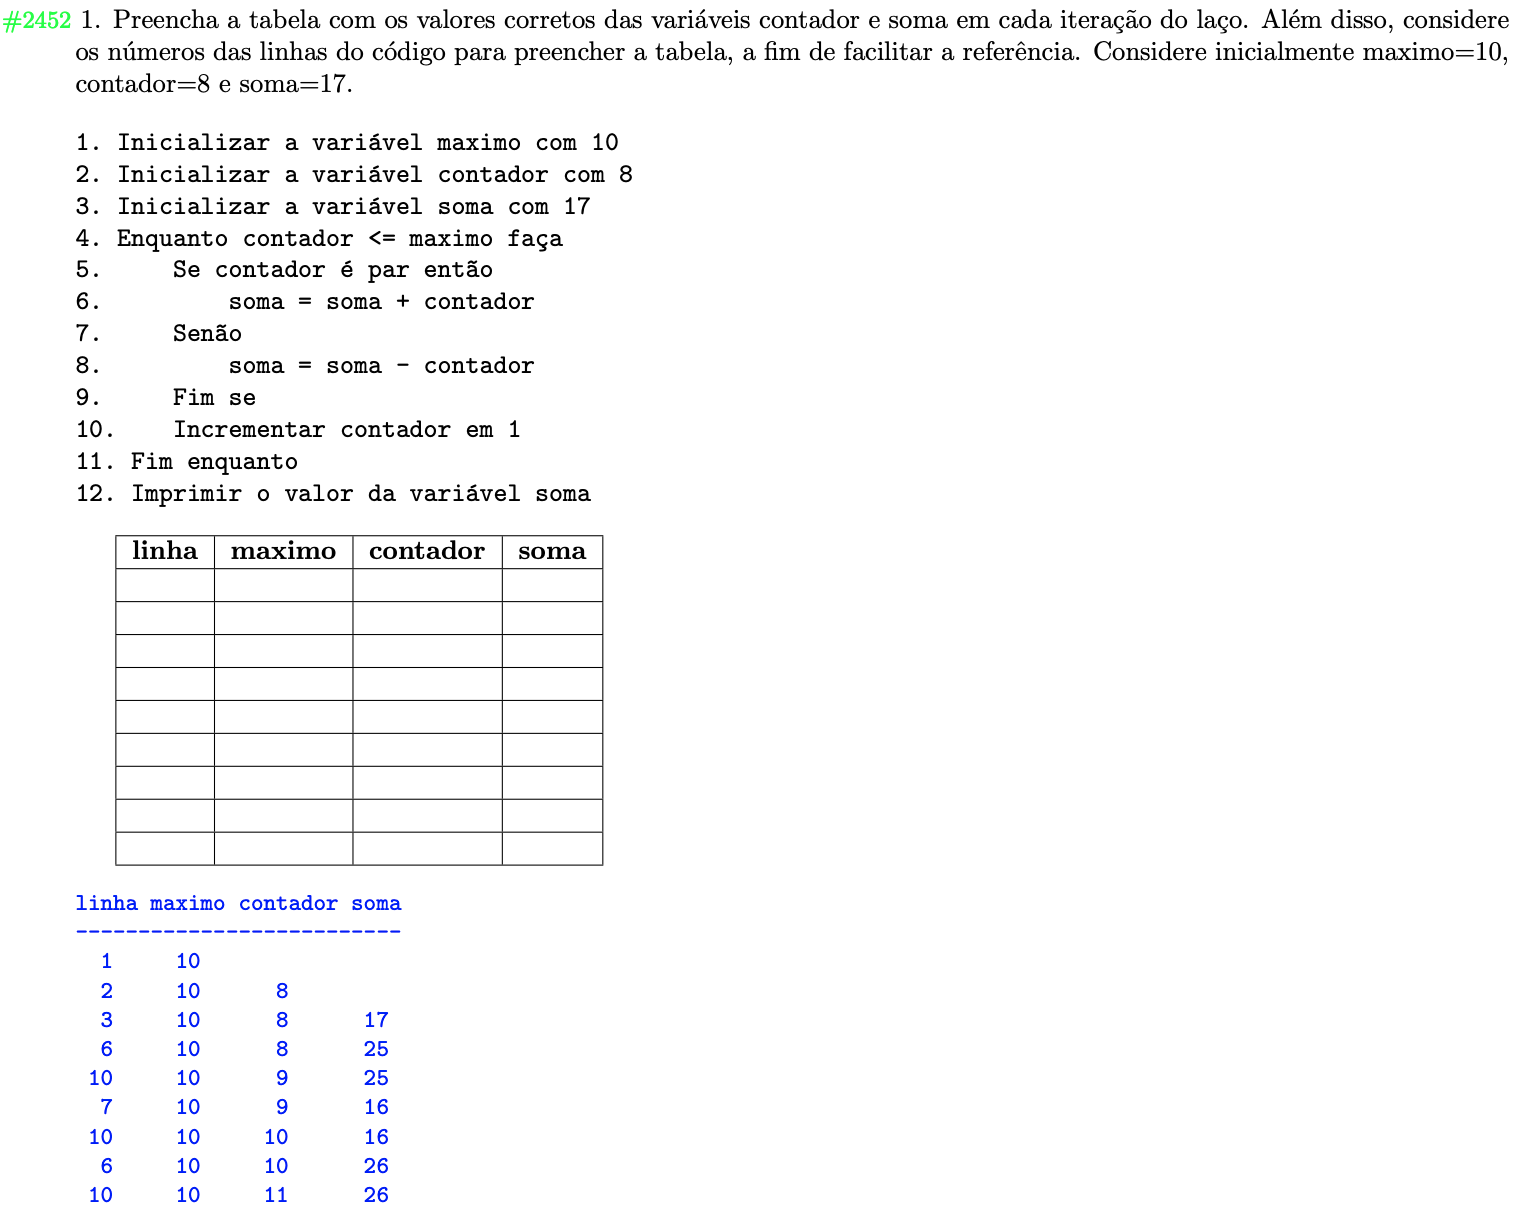
\includegraphics[width=0.9\textwidth]{cap05_questaoQT_TesteMesaEx2PDF.png}
  \caption{Recorte do PDF gerado para a questão definida no Código \ref{lst:questaoQT_TesteMesaEx2}.}
  \label{fig:cap05_questaoQT_TesteMesaEx2PDF}
\end{figure}

\subsection{Exemplo 2 -- Teste de mesa e gabarito}

É possível aprimorar o exemplo anterior expandindo-o para gerar o gabarito correspondente a cada valor aleatório gerado para as variáveis \verb|N1|, \verb|N2| e \verb|N3|. Para essa finalidade, foi criado um método em Python que implementa o algoritmo da questão. Devido à quantidade de linhas na descrição dessa questão, os códigos correspondentes foram divididos e estão disponíveis nos fragmentos dos Códigos \ref{lst:questaoQT_TesteMesaEx3Parte1} e  \ref{lst:questaoQT_TesteMesaEx3Parte2}.

Nesta nova versão, o gabarito foi adicionado ao PDF utilizando as linhas 36 a 40 do Código \ref{lst:questaoQT_TesteMesaEx3Parte1}. Na linha 36, azul e o tamanho \verb|small| foram definidos para a variável \verb|tabela|, conforme mostrado na Figura \ref{fig:cap05_questaoQT_TesteMesaEx3PDF}. Caso o professor não deseje exibir esse gabarito na folha de atividade, basta utilizar a cor \verb|white|. Na linha 38, a variável \verb|tabela|, sendo uma \textit{string}, é definida na segunda parte do código, no Código \ref{lst:questaoQT_TesteMesaEx3Parte2}.

Nesta versão, foi criado o método \verb|gerar_gabarito| para retornar a tabela atualizada para incluir as linhas específicas do algoritmo com os espaços correspondentes para preencher com os valores corretos das variáveis \verb|contador| e \verb|soma|. 

O trecho entre as linhas 27 e 31 do Código \ref{lst:questaoQT_TesteMesaEx3Parte2} apresenta um exemplo de uso do código, no qual são gerados valores aleatórios para \verb|N1|, \verb|N2| e \verb|N3| até que a tabela gerada tenha entre 10 e 15 linhas (exclusivamente). Esse trecho será analisado linha por linha:

\begin{description}
    \item \verb|while True|: isso cria um \textit{loop} infinito que será executado até que a condição na linha 30 seja satisfeita e o \textit{loop} seja interrompido na linha 31;
    \item \verb|N1, N2, N3 = random.sample(range(4, 20), 3)|: aqui é usado o método \verb|sample| da biblioteca \verb|random| para gerar três valores aleatórios, sem repetição, no intervalo de 4 a 19. Esses valores são atribuídos às variáveis \verb|N1|, \verb|N2| e \verb|N3|;
    \item \verb|tabela = gerar_gabarito(N1, N2, N3)|: o método é chamado \verb|gerar_gabarito| passando os valores aleatórios \verb|N1|, \verb|N2| e \verb|N3| como argumentos. Esse método retorna a tabela formatada com os valores corretos das variáveis \verb|contador| e \verb|soma|;
    \item \verb|if 10 < len(tabela.split('\n')) < 15: break|: aqui é verificado o número de linhas na tabela gerada. Se o número de linhas estiver entre 10 e 15 (exclusivamente), a condição é satisfeita e o \textit{loop} é interrompido com o uso do comando \textit{break}.
\end{description}

Dessa forma, esse trecho de código permite gerar valores aleatórios para as variáveis \verb|N1|, \verb|N2| e \verb|N3| repetidamente até que a tabela gerada tenha o número de linhas desejado. Isso garante que todas as variações tenham dificuldades de resolução semelhantes, testando diferentes casos. Neste exemplo simples, é possível gerar $15*15*15$ variações, mas apenas aquelas que resultarem em tabelas com 11 a 14 linhas serão consideradas.

\begin{listing}[!ht]
\begin{myboxCode}{corCodigo}{\textbf{Questão: }}\vspace{3mm}
\hrule
\begin{minted}[xleftmargin=20pt,linenos=true]{python}
Preencha a tabela com os valores corretos das variáveis contador e soma 
em cada iteração do laço.  Além disso, considere os números das linhas do 
código para preencher a tabela, a fim de facilitar a referência. Considere 
inicialmente N=[[code:N1]], contador=[[code:N2]] e soma=[[code:N3]].

\begin{verbatim}
1. Inicializar a variável N com [[code:N1]]
2. Inicializar a variável contador com [[code:N2]]
3. Inicializar a variável soma com [[code:N3]]
4. Enquanto contador <= N faça
5.     Se contador é par então
6.         soma = soma + contador
7.     Senão
8.         soma = soma - contador
9.     Fim se
10.    Incrementar contador em 1
11. Fim enquanto
12. Imprimir o valor da variável soma
\end{verbatim}

\begin{tabular}{|c|c|c|c|}
\hline
\textbf{linha} & \textbf{contador} & \textbf{soma} \\
\hline
 & & \\ \hline
 & & \\ \hline
 & & \\ \hline
 & & \\ \hline
 & & \\ \hline
 & & \\ \hline
 & & \\ \hline
 & & \\ \hline
 & & \\ \hline
\end{tabular}

{\color{blue} {\small
\begin{verbatim}
[[code:tabela]]
\end{verbatim}
}}
\end{minted}
\end{myboxCode}
\caption{Exemplo prático de teste de mesa paramétrico mostrando o gabarito -- Parte 1: Descrição de questão.}
\label{lst:questaoQT_TesteMesaEx3Parte1}
\end{listing}

\begin{listing}[!ht]
\begin{myboxCode}{corCodigo}{\textbf{Questão: }}\vspace{3mm}
\hrule
\begin{minted}[xleftmargin=20pt,linenos=true]{python}
[[def:
import random

def gerar_gabarito(N1, N2, N3):
    s = "Linha\tContador\tSoma\n"
    s += "--------------------\n"

    contador = N2
    s += f"  2 {contador:7d}\n"    
    soma = N3
    s += f"  3 {contador:7d} {soma:6d}\n"

    while contador <= N1:
        if contador % 2 == 0:
            soma = soma + contador
            s += f"  6 {contador:7d} {soma:6d}\n"
        else:
            soma = soma - contador
            s += f"  8 {contador:7d} {soma:6d}\n"

        contador += 1
        s += f" 10 {contador:7d} {soma:6d}\n"
    
    return s

# Exemplo de uso:
while True:
    N1, N2, N3 = random.sample(range(4, 20), 3)
    tabela = gerar_gabarito(N1, N2, N3)
    if 10 < len(tabela.split('\n')) < 15:
        break
]]
\end{minted}
\end{myboxCode}
\caption{Exemplo prático de teste de mesa paramétrico mostrando o gabarito -- Parte 2: Bloco de código em Python.}
\label{lst:questaoQT_TesteMesaEx3Parte2}
\end{listing}

\begin{figure}[b]
  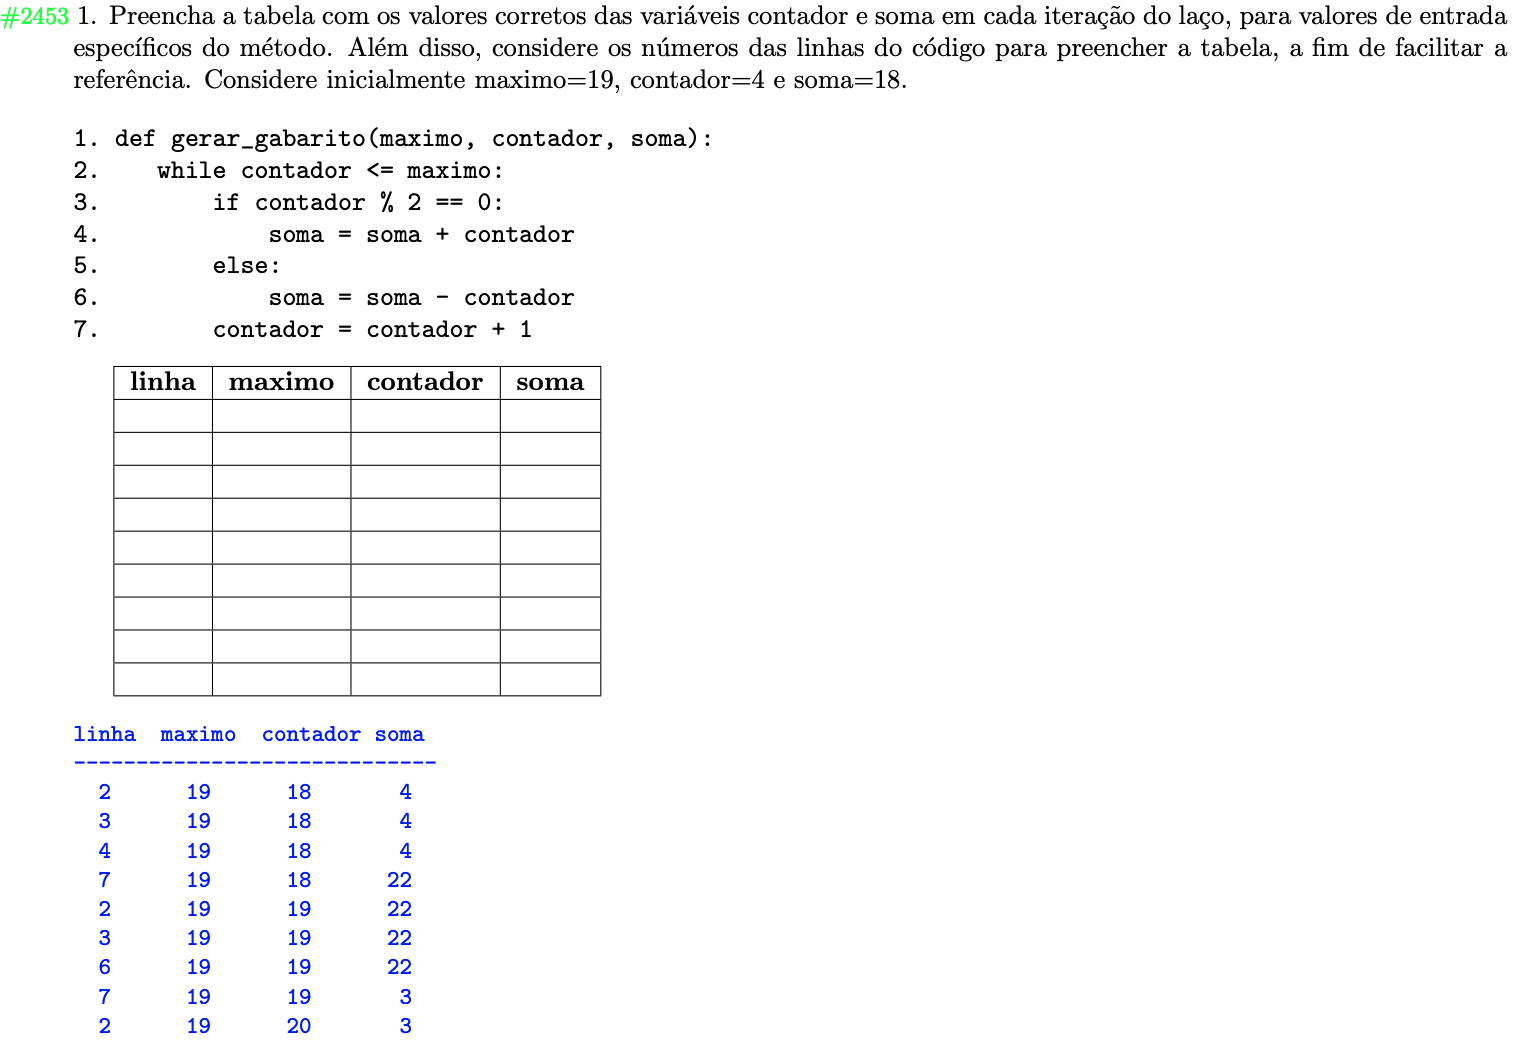
\includegraphics[width=0.9\textwidth]{cap05_questaoQT_TesteMesaEx3PDF.png}
  \caption{Recorte do PDF gerado para a questão definida nos Códigos \ref{lst:questaoQT_TesteMesaEx3Parte1} e \ref{lst:questaoQT_TesteMesaEx3Parte2}.}
  \label{fig:cap05_questaoQT_TesteMesaEx3PDF}
\end{figure}

\subsection{Exemplo 3 -- Teste de mesa e gabarito com \texttt{settrace}}
 
Um exemplo avançado de teste de mesa é o uso do método \verb|settrace| em Python. \verb|settrace| é um método da biblioteca \verb|sys| que permite definir um rastreador de ações ocorridas no código. Ele é usado para registrar um rastreamento personalizado que será chamado sempre que ocorrer uma chamada de instrução, retorno de método ou exceção.

Ao chamar \verb|sys.settrace|, é possível fornecer um rastreamento personalizado que será invocado automaticamente durante a execução do programa. Esse método de rastreamento recebe os argumentos:

\begin{description}
    \item \verb|frame|: é um objeto que representa o quadro de variáveis atual em uma pilha;
    \item \verb|event|: é uma \textit{string} que indica o tipo de evento que ocorreu. Pode ser \textit{call} (chamada de método), \textit{return} (retorno de método) ou \textit{exception} (exceção);
    \item \verb|arg|: é um argumento adicional que depende do tipo de evento. Para eventos de chamada e retorno, é sempre \textit{None}. Para eventos de exceção, é uma tupla contendo informações sobre a exceção disparada.
\end{description}

O método de rastreamento personalizado pode realizar várias ações, como exibir informações sobre as chamadas de métodos, coletar dados de execução, fazer análises dinâmicas, entre outros. É uma ferramenta poderosa para depurar e analisar o fluxo de execução de um programa Python.

É importante mencionar que o uso de \verb|sys.settrace| pode ter um impacto significativo no desempenho do programa, uma vez que o método de rastreamento é chamado em cada evento de chamada, retorno ou exceção. Portanto, é recomendado usá-lo com cuidado e apenas quando necessário para fins de depuração ou análise.

\subsubsection{Exemplo de uso do método \texttt{settrace} para rastreamento de código}

O Código \ref{lst:questaoQT_TesteMesaEx4Parte1} define o método \verb|trace| para ser chamada sempre que ocorrer um evento específico, como a execução de uma linha de código. Neste método, as informações relevantes são impressas no console, após a sua execução, como o evento, o número da linha e as variáveis locais.
%
Em seguida, o método \verb|gerar_gabarito| é definido para calcular a soma ou subtração com contador par e ímpar, respectivamente, em um determinado intervalo. O método é chamado com os argumentos 9, 7 e 6 para os parâmetros \verb|N1|, \verb|contador| e \verb|soma|, respectivamente.
%
Por fim, o método \verb|trace| é desativado na linha 16.
%
Este código é um exemplo de como usar o recurso de rastreamento em Python para depurar o código e entender como as variáveis são alteradas durante a execução. O código rastreado não possui saída, mas o rastreamento pode ser modificado para imprimir informações adicionais ou para armazenar informações em um arquivo de \textit{log}.

\begin{listing}[!ht]\vspace{-3mm}
\begin{myboxCode}{corCodigo}{\textbf{Questão: }}\vspace{3mm}
\hrule
\begin{minted}[xleftmargin=20pt,linenos=true]{python}
def trace(frame, event, arg_unused):
    print(event, frame.f_lineno, frame.f_locals)
    return trace

def gerar_gabarito(N1, contador, soma):
    while contador <= N1:
        if contador % 2 == 0:
            soma = soma + contador
        else:
            soma = soma - contador
        contador += 1

import sys
sys.settrace(trace)
gerar_gabarito(9, 7, 6)
sys.settrace(None)
\end{minted}
\end{myboxCode}
\caption{Exemplo de uso de \texttt{sys.settrace}.}\vspace{-2mm}
\label{lst:questaoQT_TesteMesaEx4Parte1}
\end{listing}\vspace{-5mm}

Ao salvar o Código \ref{lst:questaoQT_TesteMesaEx4Parte1} no arquivo \verb|trace.py| e executá-lo no console do computador usando o comando \verb|python trace.py|, a saída resultante será semelhante ao apresentado a seguir:% no Código \ref{lst:questaoQT_TesteMesaEx4Parte1saida}.

%\begin{listing}[!ht]
\begin{myboxCode}{corCSV}{\textbf{Saída do Código \ref{lst:questaoQT_TesteMesaEx4Parte1}:}}\vspace{3mm}
\hrule
\begin{minted}[xleftmargin=20pt,linenos=true]{python}
call 7 {'N1': 9, 'contador': 7, 'soma': 6}
line 8 {'N1': 9, 'contador': 7, 'soma': 6}
line 9 {'N1': 9, 'contador': 7, 'soma': 6}
line 12 {'N1': 9, 'contador': 7, 'soma': 6}
line 13 {'N1': 9, 'contador': 7, 'soma': -1}
line 8 {'N1': 9, 'contador': 8, 'soma': -1}
line 9 {'N1': 9, 'contador': 8, 'soma': -1}
line 10 {'N1': 9, 'contador': 8, 'soma': -1}
line 13 {'N1': 9, 'contador': 8, 'soma': 7}
line 8 {'N1': 9, 'contador': 9, 'soma': 7}
line 9 {'N1': 9, 'contador': 9, 'soma': 7}
line 12 {'N1': 9, 'contador': 9, 'soma': 7}
line 13 {'N1': 9, 'contador': 9, 'soma': -2}
line 8 {'N1': 9, 'contador': 10, 'soma': -2}
return 8 {'N1': 9, 'contador': 10, 'soma': -2}
\end{minted}
\end{myboxCode}
% \caption{Saída no Código \ref{lst:questaoQT_TesteMesaEx4Parte1}, ao ser executado no console do computador.}
% \label{lst:questaoQT_TesteMesaEx4Parte1saida}
% \end{listing}

É possível formatar essa saída e gerar uma questão completa no MCTest, conforme demonstrado a seguir.

\subsubsection{Teste de mesa com rastreamento de código usando \texttt{settrace}}

Neste terceiro exemplo de teste de mesa paramétrico, é utilizado o método \verb|settrace|, da biblioteca \verb|sys|, para gerar o gabarito. Este exemplo foi inspirado no artigo de \citeonline{2023:Teubl.Zampirolli}. A vantagem dessa versão em relação à anterior é que pode-se criar o gabarito sem precisar incluir vários comandos \verb|print| na implementação do pseudocódigo, tornando o processo mais genérico para diferentes exemplos de teste de mesa. A seguir, serão adaptadas as versões anteriores, criando um código em Python que faz parte do enunciado da questão, apresentado no Código \ref{lst:questaoQT_TesteMesaEx4Parte2}. No entanto, também é possível ter utilizado um pseudocódigo.

A parte com diferenças significativas em relação às anteriores é apresentada no Código \ref{lst:questaoQT_TesteMesaEx4Parte3}. Nessa parte, o método \verb|trace| é adaptado, conforme apresentado no Código \ref{lst:questaoQT_TesteMesaEx4Parte1}, para formatar a tabela com o gabarito. Dentro desse método, é verificado se o evento atual é uma linha de código (\verb|event == 'line'|). Em caso afirmativo, o método obtém o número da linha atual (\verb|lineno|) e o dicionário de variáveis locais (\verb|locals_dict|) do \verb|frame| atual.

Em seguida, o método obtém os valores das variáveis \verb|contador| e \verb|soma| do dicionário de variáveis locais, usando o método \verb|get|. Esses valores são usados para criar uma \verb|string| formatada, armazenada em uma lista chamada \verb|output|.

Por fim, o método retorna a si (\verb|return trace|), o que permite que seja chamado novamente no próximo evento de linha. Esse processo se repete até que a execução do programa seja concluída ou até encontrar o comando \verb|sys.settrace(None)|, que encerra o rastreamento.

Além disso, o código apresenta o método \verb|gerar_gabarito|, semelhante ao apresentado no Código \ref{lst:questaoQT_TesteMesaEx4Parte1}.
%
Em seguida, o trecho de código inicia um \verb|loop| infinito que realiza as seguintes ações: gera três números aleatórios distintos em um intervalo específico, inicializa uma lista vazia chamada \verb|output| e adiciona cabeçalhos e uma linha de separação à lista. Em seguida, o rastreamento do código é iniciado com \verb|sys.settrace(trace)|, o método \verb|gerar_gabarito| é executado com os valores gerados e o rastreamento é finalizado com \verb|sys.settrace(None)|. A lista \verb|output| é convertida em uma única \verb|string| chamada \verb|tabela|. O código verifica se o número de linhas na tabela está entre 11 e 14. Se a condição for satisfeita, o \verb|loop| é interrompido e o programa é finalizado. Essa estrutura de repetição permite gerar e obter uma tabela com um número específico de linhas no intervalo desejado.


% http://127.0.0.1:8000/topic/question/2453/update/
\begin{listing}[!ht]
\begin{myboxCode}{corCodigo}{\textbf{Questão: }}\vspace{3mm}
\hrule
\begin{minted}[xleftmargin=20pt,linenos=true]{python}
Preencha a tabela com os valores corretos das variáveis contador e soma 
em cada iteração do laço, para valores de entrada específicos do método. 
Além disso, considere os números das linhas do código para preencher a 
tabela, a fim de facilitar a referência. Considere inicialmente 
N1=[[code:N1]], contador=[[code:N2]] e soma=[[code:N3]].

\begin{verbatim}
1. def gerar_gabarito(N1, contador, soma):
2.    while contador <= N1:
3.        if contador % 2 == 0:
4.            soma = soma + contador
5.        else:
6.            soma = soma - contador
7.        contador += 1
\end{verbatim}

\begin{tabular}{|c|c|c|c|}
\hline
\textbf{linha} & \textbf{contador} & \textbf{soma} \\
\hline
 & & \\ \hline
 & & \\ \hline
 & & \\ \hline
 & & \\ \hline
 & & \\ \hline
 & & \\ \hline
 & & \\ \hline
 & & \\ \hline
 & & \\ \hline
\end{tabular}

{\color{blue} {\small
\begin{verbatim}
[[code:tabela]]
\end{verbatim}
}}
\end{minted}
\end{myboxCode}
\caption{Exemplo prático de teste de mesa paramétrico utilizando \texttt{sys.settrace} -- Parte 1: Descrição de questão.}
\label{lst:questaoQT_TesteMesaEx4Parte2}
\end{listing}

\begin{listing}[!ht]
\begin{myboxCode}{corCodigo}{\textbf{Questão: }}\vspace{3mm}
\hrule
\begin{minted}[xleftmargin=20pt,linenos=true]{python}
[[def:
import random, sys
global trace

def trace(frame, event, arg_unused):
    global output
    if event == 'line':
        lineno = frame.f_lineno  # pega a linha
        locals_dict = frame.f_locals  # pega todas as variáveis locais
        contador = locals_dict.get('contador')  # pega a variável contador
        soma = locals_dict.get('soma')  # pega a variável soma
        output.append(f"{lineno-16:3d} {contador:7d} {soma:7d}\n")  
        # armazena a string na lista
    return trace

def gerar_gabarito(N1, soma, contador):
    while contador <= N1:
        if contador % 2 == 0:
            soma = soma + contador
        else:
            soma = soma - contador
        contador += 1

# Exemplo de uso:
while True:
    N1, N2, N3 = random.sample(range(4, 20), 3)
    output = []
    output.append("Linha Contador Soma\n")
    output.append("---------------------\n")
    sys.settrace(trace)  # Inicializa o rastreamento
    gerar_gabarito(N1, N2, N3)
    sys.settrace(None)  # Finaliza o rastreamento
    tabela = ''.join(output)  # converte a lista de strings em uma string
    if 10 < len(tabela.split('\n')) < 15:
        break
]]
\end{minted}
\end{myboxCode}
\caption{Exemplo prático de teste de mesa paramétrico utilizando \texttt{sys.settrace} -- Parte 2: Bloco de código em Python.}
\label{lst:questaoQT_TesteMesaEx4Parte3}
\end{listing}

\begin{figure}[b]
  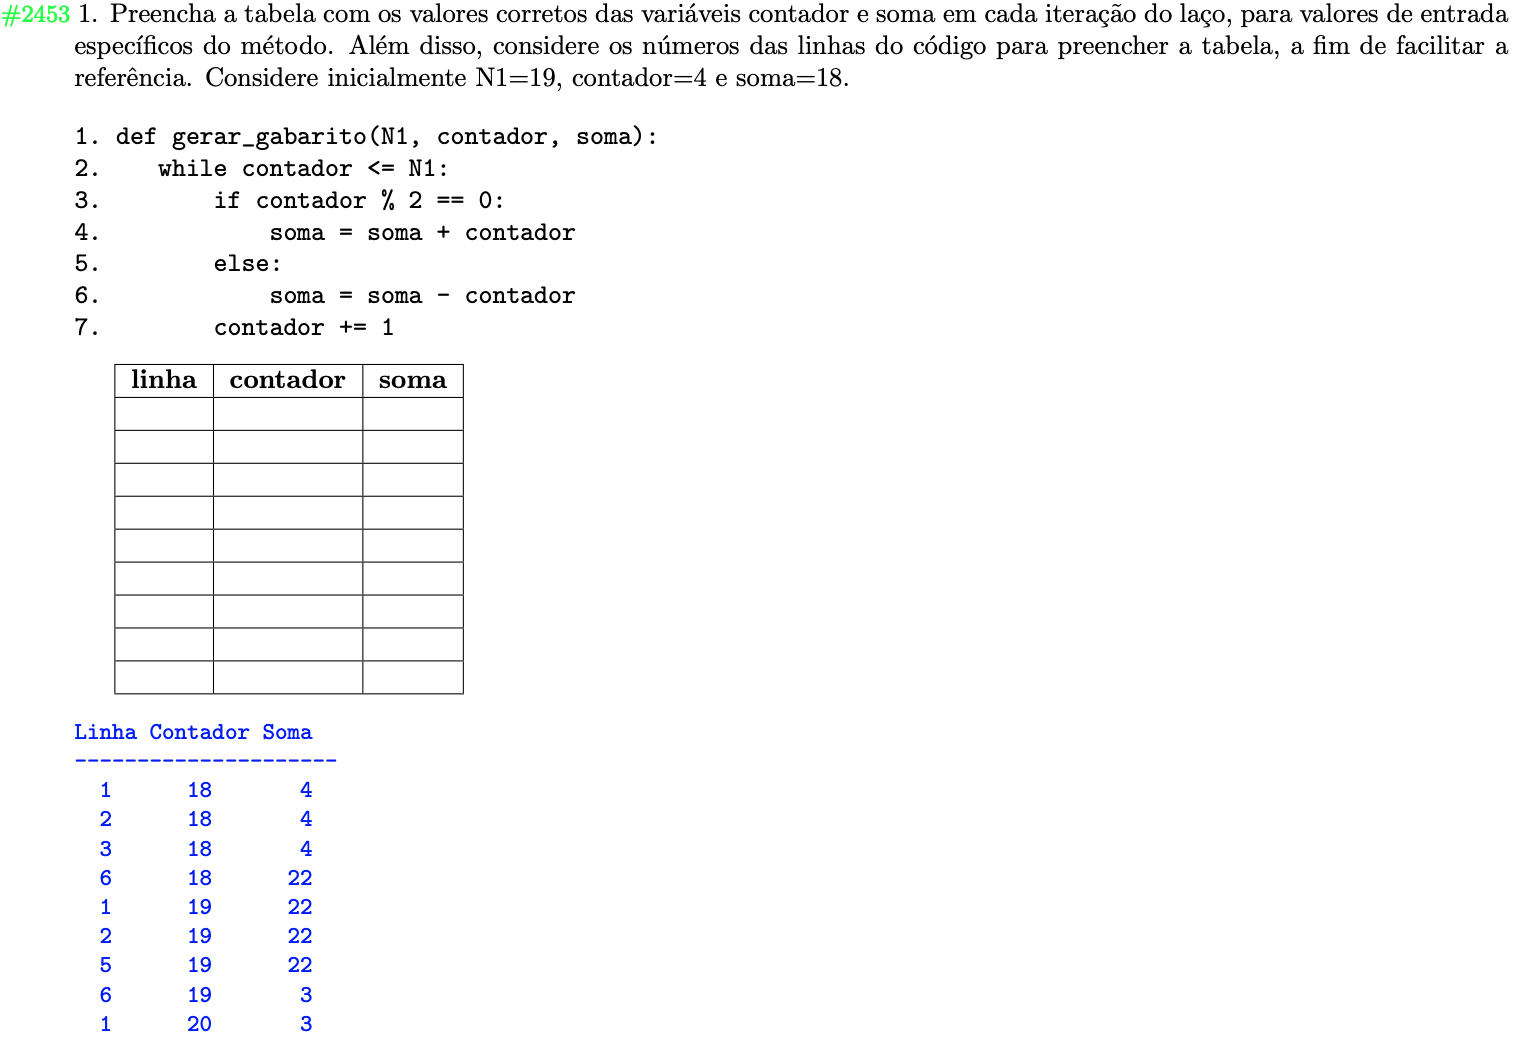
\includegraphics[width=0.9\textwidth]{cap05_questaoQT_TesteMesaEx4PDF.png}
  \caption{Recorte do PDF gerado para a questão definida nos Códigos \ref{lst:questaoQT_TesteMesaEx4Parte2} e \ref{lst:questaoQT_TesteMesaEx4Parte3}.}
  \label{fig:cap05_questaoQT_TesteMesaEx4PDF}
\end{figure}

\section{QT paramétrica, com código}\label{sec:questoesQT_VPL}

Nesta seção, são abordadas QTs paramétricas que envolvem código, introduzindo o ambiente Moodle e VPL. Em seguida, é apresentado um exemplo de atividade que combina essas duas ferramentas. Posteriormente, é fornecido um exemplo de atividade que utiliza a combinação MCTest, Moodle e VPL.

\subsection{Introdução ao Moodle e ao VPL}

O Moodle é uma plataforma de aprendizagem \textit{online} amplamente utilizada em instituições de ensino em todo o mundo. Ela oferece recursos abrangentes para apoiar o ensino e a aprendizagem, incluindo a capacidade de criar e disponibilizar atividades interativas para os estudantes. Um dos \textit{plugins} populares do Moodle é o VPL (\textit{Virtual Programming Lab}) \cite{rodriguez2012virtual}, desenvolvido especialmente para a correção automática de exercícios de programação (EPs).

O \textit{plugin} VPL permite que os professores criem EPs e ofereçam aos estudantes um ambiente virtual para escrever e testar seu código. Essa ferramenta é particularmente útil em disciplinas de programação, onde os estudantes precisam praticar e aprimorar suas habilidades de codificação.

O VPL oferece recursos avançados de avaliação e correção automática. Os estudantes podem enviar seus códigos para o sistema, e o VPL executará testes automatizados para verificar se o código produz os resultados esperados. Os resultados são fornecidos instantaneamente, permitindo que os estudantes identifiquem onde cometeram erros e onde podem melhorar.

Além disso, o VPL permite que os professores configurem casos de teste personalizados para verificar a correção dos programas dos estudantes. Isso significa que os professores podem criar uma variedade de exercícios e testes para avaliar a compreensão e a habilidade dos estudantes em diferentes aspectos da programação.

O uso do VPL no Moodle traz diversos benefícios. Ele promove a prática ativa e produz \textit{feedback} imediato aos estudantes, permitindo que eles experimentem e aprendam com seus erros. Além disso, o VPL agiliza o processo de correção, liberando mais tempo para que os professores se concentrem em fornecer orientação e apoio individualizado aos estudantes.

\subsection{Questão com exercício de programação no Moodle+VPL}

Nesta seção, será apresentada uma QT que requer a solução utilizando o \textit{
plugin} VPL do Moodle. Esse tipo de questão é definido neste livro como EP. O estudante é solicitado a inserir o código na atividade correspondente do Moodle, utilizando uma linguagem de programação definida pelo professor. É importante destacar que a questão apresentada a seguir não é paramétrica, embora possua diferentes casos de teste.

\subsubsection{Um exemplo de atividade Moodle+VPL}

Escreva um programa em Python para calcular o fatorial de um número inteiro fornecido pelo usuário.

\subsubsection{Instruções}

Aqui está um exemplo de  questão de EP no Moodle usando a linguagem Python para calcular o fatorial de um número:
\begin{enumerate}
    \item Acesse o Moodle e vá para a disciplina em que deseja adicionar a questão;
    \item Clique em ``Atividades'' e selecione ``Laboratório Virtual de Programação''  para criar uma nova atividade VPL;

    \item Preencha os detalhes da atividade, como nome, descrição e pontuação. Finalize salvando e mostrando a atividade. Em seguida, clique no ícone de engrenagem para acessar as configurações avançadas da atividade e siga os próximos passos;

    \item Na seção ``Opções de execução'', selecione a linguagem ``Python'' como ``Script de execução'', deixando apenas ``Avaliar'' e ``Atribuição automática de nota'' como ``Sim'', por exemplo;

    \item Na seção ``Casos de teste'', você pode definir os casos de teste da seguinte maneira:

\begin{myboxCode}{corCSV}{\textbf{Arquivo com os casos de teste:}}\vspace{3mm}
\hrule
\begin{verbatim}
case=caso1
input=5
output="O fatorial de 5 é 120."
output="O fatorial de 5 é 120"
case=caso2
input=10
output="O fatorial de 10 é 3628800."
output="O fatorial de 10 é 3628800"
\end{verbatim}
\end{myboxCode}

    \item Na seção ``Arquivo de execução'', você pode deixar em branco, pois não é necessário alterações neste exemplo.

\end{enumerate}

O Código \ref{lst:fatorial} apresenta um método em Python para calcular o fatorial de um número. O fatorial de um número é o produto de todos os números inteiros positivos de 1 até esse número.

O método \verb|fatorial(n)| recebe um número \verb|n| como parâmetro. Ele verifica se \verb|n| é igual a zero. Se for, retorna 1, pois o fatorial de 0 é definido como 1. Caso contrário, o método calcula o fatorial de \verb|n| multiplicando \verb|n| pelo fatorial de \verb|n-1| (ou seja, o fatorial do número anterior). Isso é feito recursivamente até chegar ao caso base do fatorial de 0.

Em seguida, o programa solicita ao usuário que digite um número inteiro. Esse número é armazenado na variável \verb|numero|. O programa então chama o método \verb|fatorial(numero)| para calcular o fatorial desse número e armazena o resultado na variável \verb|resultado|. Por fim, o programa exibe a frase \verb|"O fatorial de"| seguida do número digitado pelo usuário e do resultado calculado.

\begin{listing}[!ht]
\begin{myboxCode}{corCodigo}{\textbf{Código: } Exemplo de uso de atividade Moodle+VPL}\vspace{3mm}
\hrule
\begin{minted}[xleftmargin=20pt,linenos=true]{python}
def fatorial(n):
    if n == 0:
        return 1
    else:
        return n * fatorial(n - 1)

numero = int(input("Digite um número inteiro: "))
resultado = fatorial(numero)
print("O fatorial de", numero, "é", resultado, ".")
\end{minted}
\end{myboxCode}
\caption{Programa em Python para cálculo do fatorial.}
\label{lst:fatorial}
\end{listing}


\subsubsection{Avaliação}

A pontuação para esta questão será baseada no programa fornecido pelo estudante para ler as entradas, calcular o fatorial e produzir as saídas esperadas para os casos de teste fornecidos. Se o estudante fornecer apenas uma saída fixa, como \verb|print("O fatorial de 5 é 120.")|, a questão receberá uma nota de 50\%.

Portanto, é importante incluir uma variedade de casos de teste para avaliar corretamente o programa e identificar possíveis tentativas de trapassa. Quanto mais casos de teste forem utilizados, melhor será a avaliação, uma vez que aumenta a chance de identificar soluções corretas e detectar respostas fixas ou incorretas.


\subsection{Questão com exercício de programação no MCTest+Moodle+VPL}\label{sec:questao_VPL}

Esse tipo de questão, utilizando EP no MCTest+Moodle+VPL, apresenta dois desafios devido à falta de integração atual entre os bancos de dados do MCTest e do Moodle.

\subsubsection{Primeiro desafio}

O primeiro desafio consiste em definir a variação da atividade para cada estudante, uma vez que as atividades podem ser individuais. Para solucionar esse problema, o MCTest gera um arquivo no formato CSV chamado \verb|students_variations.csv|, contendo o nome do estudante e a variação atribuída. Esse arquivo deve ser inserido no campo ``Arquivo de execução'' da atividade VPL no Moodle. Além disso, existem vários outros arquivos disponíveis no GitHub, detalhados em capítulos futuros deste livro, que também devem ser incluídos nesse campo. A versão utilizada neste livro está na pasta \href{https://github.com/fzampirolli/mctest/tree/master/VPL_modification}{\texttt{V10-new\_selector}} do GitHub.

\begin{mybox}{corCopia}{\textbf{Atenção:\\\vspace{-3mm}\hrule\vspace{3mm}}}
É importante destacar que a busca pela variação do estudante deve ser realizada pelo nome e sobrenome do estudante no arquivo \verb|students_variations.csv|, sendo necessário que esses dados sejam idênticos tanto no MCTest quanto no Moodle. Em versões recentes do VPL, também é possível utilizar o e-mail do estudante, o que representará uma melhoria futura nesse processo.
\end{mybox}

\subsubsection{Segundo desafio}

O segundo desafio, ainda mais crítico, envolve a definição dos casos de teste para cada variação da questão. Esse desafio é enfrentado através da geração do arquivo \verb|linker.json| pelo MCTest, no formato JSON. Esse arquivo contém as variações da atividade, incluindo as questões e seus respectivos casos de teste. Nesta seção, será abordado o processo de criação de uma QT paramétrica de EP no MCTest+Moodle+VPL. No entanto, é importante ressaltar que todos os detalhes desse processo serão abordados em capítulos futuros, uma vez que os arquivos CSV e JSON são gerados ao criar um exame no MCTest, especificamente no Capítulo \ref{ch:examesQT_VPL} -- \nameref{ch:examesQT_VPL}.

\subsubsection{Um exemplo simples de cálculo de parcelas sem juros}

O VPL considera cada linha como uma entrada de dados de um programa. No Python, essa entrada é capturada utilizando o comando \verb|input()|, que recebe um texto. Por exemplo, o texto \verb|"5003.9\n10\n"| contém duas entradas. Para uma questão de parcelas sem juros, é possível ter duas entradas e uma saída de dados no Código \ref{lst:parcelasSemJuros} em Python, que pode ser testado em uma atividade VPL no Moodle.
%
\begin{listing}[!ht]
\begin{myboxCode}{corCodigo}{\textbf{Código: } Exemplo de uso de atividade Moodle+VPL -- Parcelas}\vspace{3mm}
\hrule
\begin{minted}[xleftmargin=20pt,linenos=true]{python}
valor_total = float(input())
parcelas = int(input())

valor_parcela = valor_total / parcelas

print(f"{valor_parcela:.2f}")
\end{minted}
\end{myboxCode}
\caption{Programa em Python para cálculo de parcelas.}
\label{lst:parcelasSemJuros}
\end{listing}
%
Nesse exemplo, o programa captura o valor total e o número de parcelas informados pelo usuário e calcula o valor de cada parcela. Em seguida, exibe o resultado utilizando o comando \verb|print|, formatando com duas casas decimais.

O MCTest pode gerar automaticamente diversos casos de teste, seguindo uma estrutura específica de dicionário de dados. Por exemplo, a seguir estão apresentados dois casos de teste criados no MCTest para o exemplo de cálculo de parcelas sem juros:

\begin{myboxCode}{corCSV}{\textbf{Dicionário usado no MCTest contendo os casos de teste:}}\vspace{3mm}
\hrule
\begin{verbatim}
moodle_cases = {
  "input": ["5009.4\n10\n", "5003.9\n10\n"],
  "output": ["500.94", "500.39"]
}
\end{verbatim}
\end{myboxCode}

Esse dicionário será formatado no arquivo \verb|linker.json|, que será tratado por vários arquivos que deverão ser inseridos em ``Arquivos de execução'', em uma atividade VPL no Moodle, que pode ser equivalente aos seguintes casos de teste.

\begin{myboxCode}{corCSV}{\textbf{Arquivo com os casos de teste:}}\vspace{3mm}
\hrule
\begin{verbatim}
case=caso1
input=5009.4
10
output=500.94
case=caso2
input=5003.9
10
output=500.39
\end{verbatim}
\end{myboxCode}

Para realizar essa tarefa, na descrição da questão no MCTest, é necessário incluir um trecho de código utilizando o comando \verb|comment| que contenha apenas o dicionário de casos de teste. Esse trecho indica ao gerador MCTest para incluir os casos de teste no arquivo \verb|linker.json|, que será importado no Moodle.

\subsubsection{Criando uma QT paramétrica para integração MCTest+Moodle+VPL}

A seguir, será apresentado um exemplo completo de código para essa questão de parcelas sem juros, onde as variáveis e instruções em Python estão entre os marcadores \verb|[[code:| e \verb|]]|. Essas variáveis devem ser criadas no bloco de código Python definido entre os marcadores \verb|[[def:| e \verb|]]|.

Para criar questões paramétricas, não apenas nos casos de teste, é necessário incluir variáveis aleatórias no enunciado da questão entre \verb|[[code:| e \verb|]]|. No exemplo das parcelas sem juros, foi incluído no enunciado o número de parcelas, sendo utilizado apenas o valor da compra como entrada para o caso de teste.


\begin{mybox}{corCopia}{\textbf{Atenção:\\\vspace{-3mm}\hrule\vspace{3mm}}}
Para garantir que cada estudante receba uma questão diferente, é necessário incluir o maior número possível de variáveis aleatórias no enunciado. Por exemplo, ao lidar com um problema de parcelas sem juros, é possível adicionar variáveis aleatórias como o nome do cliente, o produto em questão, entre outros. Além disso, é importante que esses dados sejam impressos na saída esperada para os casos de teste. Caso contrário, um mesmo código pode funcionar para todas as variações de atividade, ignorando a necessidade de múltiplos casos de teste.
\end{mybox}

No Código \ref{lst:questaoQT_EP_1_parte1}, é apresentado o enunciado da questão, incluindo a parcela como parte paramétrica. Também é incluído o primeiro caso de teste como exemplo no enunciado. Essa primeira parte é finalizada com o bloco \verb|comment|, necessário para o MCTest entender que se trata de uma questão onde o estudante deve resolver como uma atividade VPL no Moodle.


\begin{listing}[!ht]
\begin{myboxCode}{corCodigo}{\textbf{Questão: }}\vspace{3mm}
\hrule
\begin{minted}[xleftmargin=20pt,linenos=true]{python}
Escreva um programa que auxilia uma loja na hora de efetuar uma venda. Seu 
programa deve perguntar o preço do produto e considerar que a loja parcela 
este preço em somente em  [[code:parcelas]] parcelas (sem juros).  O seu 
programa deve mostrar quanto será o valor de uma parcela (arredondando 
para duas casas decimais apenas). Veja exemplo a seguir: \\

\noindent\textbf{Exemplo de Entrada:}
\begin{verbatim}
[[code:caso0_inp]]
\end{verbatim}

\noindent\textbf{Exemplo de Saída:}
\begin{verbatim}
[[code:caso0_out]]
\end{verbatim}

% necessário para gerar casos de testes no moodle
\begin{comment}
[[code:moodle_cases]]
\end{comment}
\end{minted}
\end{myboxCode}
\caption{Exemplo de QT paramétrica utilizando MCTest+Moodle+VPL -- Parte 1: Descrição de questão.}
\label{lst:questaoQT_EP_1_parte1}
\end{listing}


A segunda parte da questão apresentada no Código \ref{lst:questaoQT_EP_1_parte1} é fornecida no Código \ref{lst:questaoQT_EP_1_parte2}, que contém o bloco de código Python que define a parte paramétrica, incluindo o dicionário \verb|moodle_cases| que contém os casos de teste.

O Código \ref{lst:questaoQT_EP_1_parte2} consiste em quatro passos principais. No Passo 1, um número inteiro aleatório entre 8 e 19 é gerado, representando o número de parcelas em uma QT paramétrica. No Passo 2, os casos de teste são criados. Para cada caso de teste, um valor aleatório para o preço do produto é gerado e as entradas e saídas correspondentes são formatadas. No Passo 3, um dicionário contendo os casos de teste é criado e convertido para o formato JSON. Por fim, no Passo 4, um exemplo de caso de teste é mostrado no enunciado da questão. Esse código permite gerar casos de teste e parâmetros para questões paramétricas, proporcionando variação nos valores dos testes e facilitando a criação de questões personalizadas. É importante testar o código em uma IDE antes de utilizá-lo no MCTest.

\begin{mybox}{corCopia}{\textbf{Atenção:\\\vspace{-3mm}\hrule\vspace{3mm}}}
Dentre os quatro passos apresentados, o professor precisa apenas modificar o Passo 1, onde os parâmetros do enunciado da questão são definidos. Além disso, o trecho entre \verb|#>>>>| e \verb|#<<<<| deve ser alterado para criar diferentes casos de teste. Essas modificações permitem criar outras questões paramétricas, com variações nos parâmetros e nos casos de teste, tornando o processo de criação mais flexível e personalizado.
\end{mybox}


\begin{listing}[!ht]
\begin{myboxCode}{corCodigo}{\textbf{Questão: } }\vspace{3mm}
\hrule
\begin{minted}[xleftmargin=20pt,linenos=true]{python}
[[def: 
# Antes de prosseguir, é recomendado testar o trecho de código  
# Python a seguir em uma IDE para garantir seu funcionamento correto.
import json
import numpy as np # uso da biblioteca numpy para gerar número aleatório 

# Passo 1: Criar os parâmetros do enunciado da questão
parcelas =  np.random.randint(8,20)

# Passo 2: Criar os casos de teste
inp_list, out_list = [], []  # Listas vazias para armazenar os casos de teste
casos_teste = 2  # Número de casos de teste desejado
# Aumentar esse número após validar a questão também na atividade VPL do Moodle

# Para cada caso de teste:
for i in range(casos_teste):    

    #>>>> begin - casos de teste
    # Gerar um valor aleatório para o preço do produto
    valor_total = np.random.randint(100)/10 + 5001 

    # Criar a entrada do caso de teste como uma string
    inp = str(valor_total)+'\n'

    # Calcular o valor da parcela arredondado para duas casas decimais
    out = f'{(valor_total/parcelas):.2f}'
    #<<<< end - casos de teste

    # Adicionar a entrada e saída do caso de teste às listas
    inp_list.append(inp)
    out_list.append(out)

# Passo 3: Criar o dicionário com os casos de teste
cases = {}
cases['input']  = np.array(inp_list).tolist()
cases['output'] = np.array(out_list).tolist()
moodle_cases = json.dumps(cases)

# Passo 4: Mostrar um exemplo no enunciado da questão
caso0_inp = cases['input'][0]
caso0_out = cases['output'][0]

#print(moodle_cases) # para testar em uma IDE
]]
\end{minted}
\end{myboxCode}
\caption{Exemplo de QT paramétrica utilizando MCTest+Moodle+VPL -- Parte 2: Bloco de código em Python.}
\label{lst:questaoQT_EP_1_parte2}
\end{listing}

Veja o resultado desta questão criada no MCTest após clicar em ``Criar-PDF'' na Figura \ref{fig:cap05_questaoQT_EP_1}. Observa-se que, na descrição da questão, é exibido \verb|Integration: Moodle+VPL|, indicando que o MCTest reconheceu essa questão como uma tarefa que o estudante deve realizar em uma atividade VPL no ambiente do Moodle, devido ao reconhecimento do comando \verb|command| no enunciado da questão.

\begin{figure}[b]
  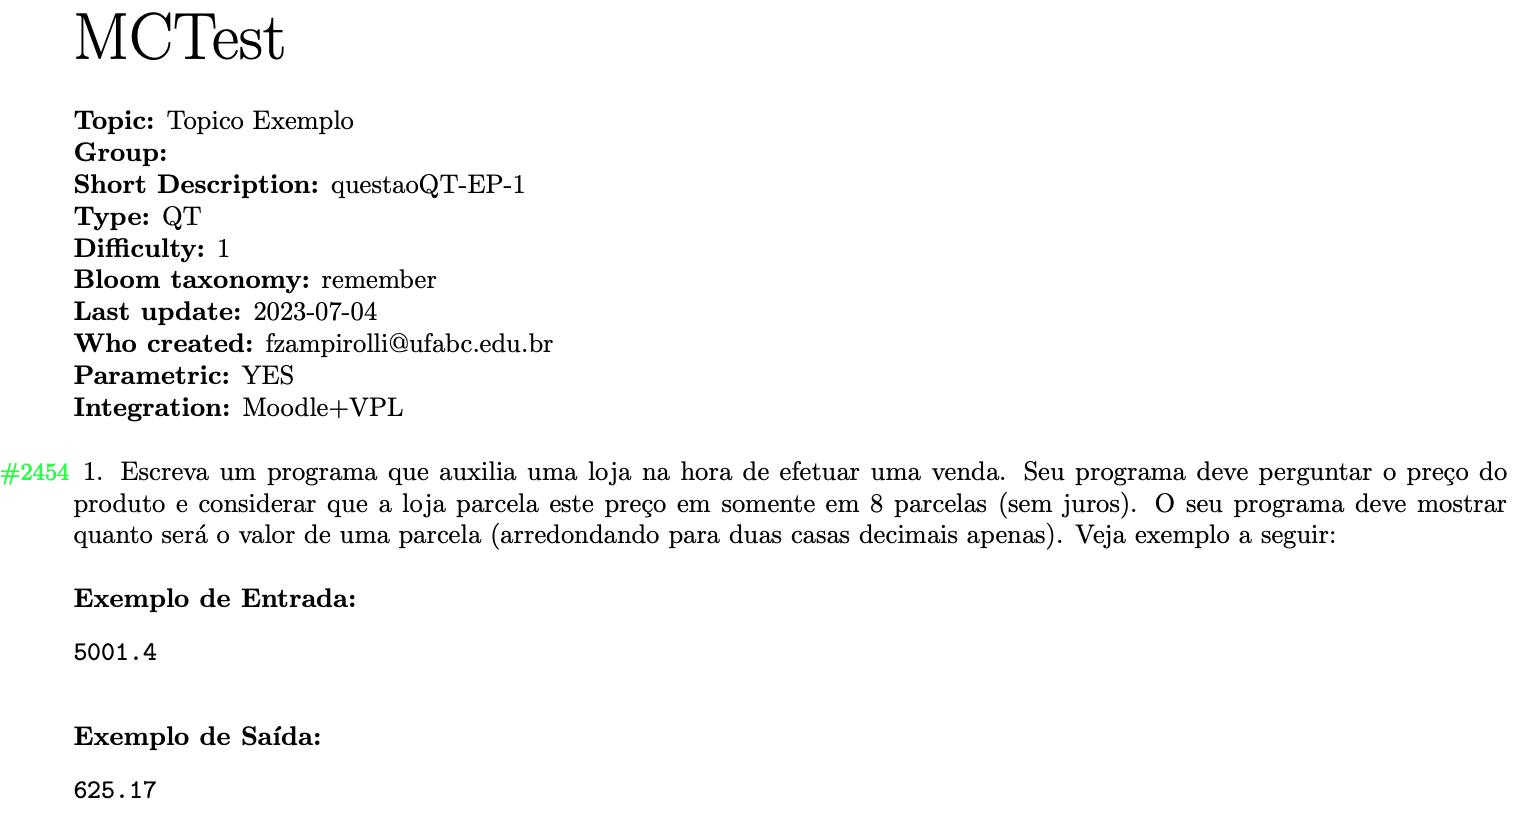
\includegraphics[width=0.9\textwidth]{cap05_questaoQT_EP_1.png}
  \caption{Recorte do PDF gerado para a QT definida nos Códigos \ref{lst:questaoQT_EP_1_parte1} e \ref{lst:questaoQT_EP_1_parte2}.}
  \label{fig:cap05_questaoQT_EP_1}
\end{figure}


\section{Considerações finais}

Neste capítulo, foram exploradas algumas possibilidades de criação de questões paramétricas no MCTest, combinando recursos de \LaTeX{} e Python. Foram apresentados exemplos simples, mas é importante ressaltar que é possível criar questões paramétricas muito mais complexas, dependendo da criatividade do professor. Essa capacidade de criação personalizada é uma das partes mais importantes do MCTest, ao permitir a geração e compartilhamento de questões para os mais diferentes fins.

Embora a criação de questões paramétricas possa exigir habilidades de programação por parte dos professores, o MCTest oferece a vantagem de gerenciar avaliações com um banco de questões reutilizáveis. Isso é especialmente útil quando há um grupo de professores interessados e uma grande demanda de avaliações para milhares de estudantes. 

No caso das QMs paramétricas, foram apresentados exemplos de como criar questões com variações de parâmetros, permitindo a geração fácil e rápida de inúmeras questões. Também foram discutidas diferentes técnicas de parametrização, oferecendo ao professor a liberdade de escolher a que melhor se adapta às suas habilidades de programação.

Em relação às QTs paramétricas, foram destacados que os conceitos e técnicas apresentados para as QMs também se aplicam a esse tipo de questão. No entanto, nas QTs, não é preciso se preocupar com as alternativas. Foram apresentados exemplos de questões paramétricas onde os parâmetros foram variados, permitindo uma ampla gama de variações para os estudantes.

Por fim, foram abordadas QTs paramétricas que envolvem código e introduzido o ambiente Moodle e o \textit{plugin} VPL. Mostrou-se como criar questões de EPs utilizando o Moodle+VPL e discutiram-se os benefícios dessa abordagem, incluindo a prática ativa, o \textit{feedback} imediato e a agilidade na correção. Também foram mencionados os desafios de integrar o MCTest, Moodle e VPL para questões paramétricas de EP. A combinação dessas ferramentas oferece aos professores uma poderosa maneira de criar e avaliar questões paramétricas personalizadas, enriquecendo a experiência de aprendizagem dos estudantes.